\chapter{Session attacks}\label{attacks}

Now that we know how web sessions work, we look into ways in which attackers are able to abuse them. In this chapter, we will see how an attacker can use the concept of web sessions to impersonate a legitimate user on a website.

\section{Background: cross-site scripting}\label{xss}

Cross-site scripting (or \gls{xss}) is not a session attack in itself. Instead, it is the exploitation of a vulnerability in some websites which can be of great use when executing one of the other attacks described below.

In a cross-site scripting attack, the attacker exploits a vulnerability in a website to inject his own JavaScript code into this page \cite{DiLucca2005}. The code will then be executed in the browser of any user that loads the page with the injected code.

\subsection{Variants of cross-site scripting}
There are two forms of cross-site scripting: persistent and non-persistent XSS. In this subsection, we describe their differences and give some examples of possible attack scenarios for each of them.

\subsubsection{Persistent (stored) XSS}
In a persistent attack, the attacker makes the web application store the script code in a database. The complete scenario goes as follows:

\begin{enumerate}
	\item The attacker provides his malicious code as input to the web application.  The web server stores this input (and thus the script code) in the database to be able to provide it to clients later on.
	\item The victim requests a page containing content generated by the attacker. The server returns the page containing the attacker's JavaScript.
	\item The victim's browser thinks that the script code is part of the requested web page and executes it.
\end{enumerate}

This attack variant is graphically illustrated in figure \ref{fig:persistent-xss}.

\begin{figure}[ht]
	\centering
	\subfloat[persistent]{
		\label{fig:persistent-xss}
		\includegraphics[width=.45\textwidth]{img/persistent-xss.png}
	}
	\subfloat[non-persistent]{
		\label{fig:nonpersistent-xss}
		\includegraphics[width=0.45\textwidth]{img/nonpersistent-xss.png}
	}
	\caption{The cross-site scripting attack}
\end{figure}

An example of a web application that will store user input in a database to serve it later it is a bulletin board (phpBB\footnote{\url{http://www.phpbb.com/}} is a well-known example), where a user can create forum posts that will be read by other users of the bulletin board. When an attacker inserts script code into a post, the code will be executed at the browser of every user reading that post.

A more recent example is found in social networking sites like Facebook\footnote{\url{http://www.facebook.com}}. Here, a user can place information on his own page, or the pages of other people. This information will then be served to the user's friends.
% Image

\subsubsection{Non-persistent (reflected) XSS}
In a non-persistent attack, the script code is never stored at the server side. Instead, code that was part of a request is immediately reflected back to a client's browser as part of the response page. The steps are as follows:

\begin{enumerate}
	\item The attacker tricks the victim into opening a malicious link containing script code.
	\item The victim opens the link, and unknowingly makes a request containing script code to the server.
	\item The server reflects this script code back to the victim as part of the response.
	\item The victim's browser thinks that the script code is part of the requested web page and executes it.
\end{enumerate}

This attack variant is graphically illustrated in figure \ref{fig:nonpersistent-xss}.

An example of this is a search form, where a website returns the term the user searched for, without stripping any script data that might be inside. If doing a search by going to the URL \url{http://www.trusted.com/search?q=searchterm} makes the website return ``x results for \emph{searchterm}'', the attacker can replace \emph{searchterm} by script code that will execute at the client that loads the search results. The attacker can then trick a user into clicking the link, causing the JavaScript code to be executed in his browser.

Another example of a scenario where a website might return data found in the URL is the `Page not found' error page \cite{Kirda2006}. Here, the name of the page that could not be found is often included as part of the error message. Thus, an attacker can craft a link wherein he requests a page with name \texttt{<script>alert("XSS succeeded");</script>} to make a client's browser execute JavaScript code.
% Image

\subsection{Including the script code}\label{injecting-script}
There are multiple ways in which script code can be included in a web page. Since all of these can be leveraged by an attacker to inject his code into a web page, it is important that web developers are aware of all of them. T. Jim et al. give a good overview of different approaches to including JavaScript code \cite{Jim2007}, of which we will describe the most important ones here:
\begin{description}
	\item[between \texttt{<script>} tags] This is the most obvious way of including JavaScript in a web page. All code between these tags will be executed as soon as the browser encounters it.
	\item[using the \texttt{<script>} tag's \texttt{source} parameter] This parameter can be set to point to an external piece of JavaScript. As such, an attacker is able to make a website load JavaScript code from another domain. An advantage for the attacker is that the actual injected string is shorter, bypassing message length limits.
	\item[as the URL of the background image] An attacker can insert a tag similar to \texttt{<div style="background-image: url(javascript:alert('XSS');" />} or \texttt{<style>.bar\{background-image:url("javascript:alert('XSS');");\}</style>} (where \texttt{bar} is the class of an object in the page) to make the browser execute JavaScript, thinking it is loading the background image.
	\item[using the \texttt{onload} parameter of the \texttt{<body>} tag] This tag is used for code that should be executed once the browser has completed loading the page.
\end{description}

It must also be noted that attackers can use different possible encodings to inject JavaScript, so as to circumvent server-side JavaScript checkers, while still being able to execute at the client side \cite{Jim2007}. For example, the encoding of (parts of) a web page can be changed using the \texttt{encoding} and \texttt{charset} attributes of various HTML tags \cite{Ishida2010}. Some browsers also allow strings to contain JavaScript that is split over multiple lines \cite{Jim2007}. Lastly, JavaScript can be split over multiple  \texttt{<![CDATA[\dots]]>} tags, making it much harder to detect.

\subsection{The danger of cross-site scripting}\label{xss-problem}

One danger of persistent XSS is immediately clear: websites that do not belong to an attacker can still be used by the attacker to execute malicious code at a user's browser. The user, thinking that a known site will only execute trusted code, can fall victim to the attacker without expecting it.

There is, however, a bigger problem which applies to both persistent and non-persistent XSS: the problem of trust. Normally, the attacker's code would be subject to the \gls{sop} (described in section \ref{sop}), making him unable to access elements of a domain that he does not own. However, when the attacker's code is able to execute from within a trusted domain (as is the case in an XSS attack), this code may access the elements belonging to the trusted domain \cite{Klein2002}. This gives the attacker the ability to read information from, and write information to, elements in the trusted domain.

The situation is even worse when the attacker's code is loaded from a different domain (because the attacker injected the script code by using the \texttt{<script>} tag's \texttt{src} attribute, for example). When this is the case, the script code is also allowed to communicate with the domain it was loaded from \cite{Singh2010}, i.e. the attacker's domain. Because of this, the attacker is able to capture information from a trusted domain and subsequently send this information to his own domain. This will be a major attack vector for the session hijacking and session fixation attacks, as we will see in the next sections.

\section{Session hijacking}\label{hijacking}

In the session hijacking attack, an attacker tries to take over a victim's session by capturing his \gls{session id}. Using this SID, the attacker can make the server think that he is the victim. First, we describe the attack scenario. Afterwards, we will see how the attacker can capture the victim's session ID.

\subsection{Attack scenario}

The session hijacking attack works as follows \cite{Nikiforakis2010}:

\begin{enumerate}
	\item The victim establishes a new session at the server. This is done automatically by the victim's browser either when he first visits the page or when he logs in (depending on the web application).
	\item The attacker captures the session ID that corresponds to the victim's created session by using one of the methods described in section \ref{capturing}.
	\item The attacker makes a request to the server, attaching the captured session ID as his own. Because the server has no other means of distinguishing between the victim and the attacker, it thinks that it is the victim that made the request. Thus, the attacker is now able to impersonate the victim at the server.
\end{enumerate}

These steps are graphically illustrated in figure \ref{fig:hijacking}.

\begin{figure}[ht]
	\centering
	\includegraphics[width=0.50\textwidth]{img/hijacking.png}
	\caption{The session hijacking attack}
	\label{fig:hijacking}
\end{figure}

\subsection{Capturing the session ID}\label{capturing}

There are lots of possible ways in which an attacker can capture a victim's session ID. We list the most important ones here.

\subsubsection{Via a (passive) man-in-the-middle attack}

In a man-in-the-middle (or \gls{mitm}) attack, an attacker is able to read traffic that passes between the client and the server. This is usually the case because both the client and the attacker are using the same network unencrypted WiFi network, or because they share the same network hub.

The session identifier is, by default, sent over the network as an unencrypted string of text, both when using cookies as when making use of URL rewriting. Because of this, an attacker able to read all network traffic can easily extract the SID from the \texttt{Cookie} header in one of the user's requests, or even from the \texttt{Set-Cookie} header in the server response setting the cookie \cite{Adida2008}.

This problem has been known for some time, and has recently again received some attention thanks to tools like Hamster \cite{Graham2007} and Firesheep \cite{Butler2010}, which make a session hijacking attack almost trivial when the victim is on an insecure network.

\subsubsection{Via cross-site scripting}

The \gls{xss} attack described in section \ref{xss} can also be used to steal a victim's session ID. For this, the attacker uses the \texttt{<script>} tag's \texttt{src} attribute to load script code from his own domain into a web page on the domain he wants to acquire the cookie from. Because the script code is loaded from within a page on the target domain, the attacker has access to both the target domain's cookie via the \texttt{cookie} attribute of the \texttt{domain} \gls{dom} object (for SIDs set in cookies), and to all links on the current page (for SIDs used via URL rewriting). However, since the script code was loaded from the attacker's domain, it is also allowed to communicate to that domain (see section \ref{xss-problem} and \cite{Klein2002} for more information). Because of this, the attacker is able to forward the target domain's cookie to his own domain, effectively capturing the client's SID.

\subsubsection{Via the referer header}

A third possible SID leak occurs when the browser attaches the \texttt{referer} header to a request going to another domain \cite{Fu2001}. The \texttt{referer} header is used to transmit the resource from which the request-URL was obtained \cite{rfc2616}. If SIDs are included in the URL (as is the case with URL rewriting), the website receiving the \texttt{referer} header as part of the request can extract the client's SID for the web application that contained the link.

If, for example, a social networking website manages sessions via URL rewriting, an attacker could share a link to his own website on this website. When another user clicks the link, a request is made to the attacker's web server. This request contains the URL of the current page, and thus the user's SID for the social networking website, in the \texttt{referer} header, making it available to the attacker.

Sometimes, the \texttt{referer} header is suppressed in the network or by the browser, especially for cross-domain requests \cite{Barth2008}. Unfortunately, the percentage of requests where the \texttt{referer} header is stripped is still small enough to consider leaking of SIDs via this channel a significant threat.

\subsubsection{Via the user}

Lastly, it is also possible that the user unknowingly leaks his own session identifier. This is the case when the user shares a link to a page for a website that uses URL rewriting \cite{Johnston2004}, for example via email or a social networking site. When another user clicks the shared link, he will automatically take over the first user's session. Thus, the second user essentially performs a session hijacking attack on the first user, possibly without even realizing it.

This problem, together with the possibility of leaking SIDs via the \texttt{referer} header, provides a strong argument against using URL rewriting for session management.

\section{Session fixation}\label{fixation}

In the session fixation attack, as in the \gls{session hijacking} attack (section \ref{hijacking}), an attacker's goal is to be using the same session as a victim. However, instead of capturing the victim's \gls{session id}, the attacker forces the victim to use a SID that is known in advance. We will first describe the steps necessary to execute this attack. Afterwards, we list the ways in which the attacker can force a victim to use a certain session ID.

\subsection{Attack scenario}

The session fixation attack works as follows \cite{Kolsek2002}:

\begin{enumerate}
	\item The \emph{attacker} establishes a new session at the server. He does this by sending a request that doesn't include a SID. The server will then attach a newly generated
SID to the response. Some servers also accept random SIDs\footnote{By random SIDs, we mean that these SIDs don't need to be generated by the server in advance. A random SID can be sent by the client on his first request.} \cite{Shiflett2004}. If this is the case, the attacker can just make up a new SID, and no request needs to be made.
	\item The attacker forces the victim to use the newly created session ID. We will see how this can be done in section \ref{injecting-sid}.
	\item The victim uses his credentials to log in at the server. The SID that was injected at the client's web browser will automatically be attached to the request. Because of this, there now exists a session at the server in which the victim is logged in. That session is identified by a SID which is known by the attacker.
	\item The attacker makes a request to the server, attaching the captured session ID as his own. This makes the server think that it is the victim that made the request. Thus, the attacker is now able to impersonate the victim at the server.
\end{enumerate}

These steps are graphically illustrated in figure \ref{fig:fixation}.

\begin{figure}[ht]
	\centering
	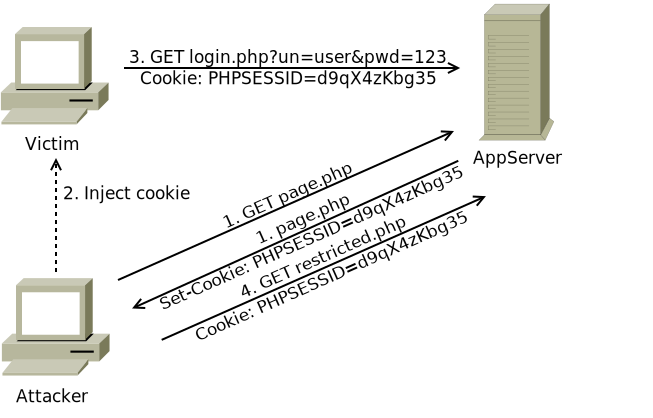
\includegraphics[width=0.50\textwidth]{img/fixation.png}
	\caption{The session fixation attack}
	\label{fig:fixation}
\end{figure}

\subsection{Injecting a session ID}\label{injecting-sid}

In this section, we describe the most important attack vectors the attacker can use to inject a session ID into the victim's browser.

\subsubsection{Via GET or POST parameters}

If the target website accepts session ID's in \glspl{url} (see section \ref{session-management}), the attacker can craft a link of the form \url{http://www.target.com/login.php?PHPSESSID=d9qX4zKbg35}, where he chooses the desired session ID \cite{Johns2011}. He then sends this link to the victim, or places on the target website as part of a \gls{xss} attack. When the victim clicks the link, the request sent to the target server will contain the attacker's SID in the URL, causing the web application to think it is the victim's session ID. Alternatively, the attacker can force the victim to visit the URL by using a HTTP redirect \cite{rfc2616} to make the victim's browser automatically load the page \cite{Shiflett2004}. However, this requires the attacker to be able to perform a XSS attack, or the victim to visit the attacker's page.

In case the target website uses POST instead of GET parameters for session management, the link can be replaced by an automatically submitting form \cite{Kolsek2002,Bontrager2005}.

Note that, for a website to accept session IDs via GET or POST parameters, it doesn't have to do its session management via URL rewriting by default. Indeed, multiple frameworks provide URL rewriting as a fallback for browsers that don't support cookies, causing them to be vulnerable to session fixation via URL rewriting \cite{Condit2006,Holovaty2008}.

\subsubsection{Via cross-site scripting}

If an attacker is able to inject script code into the target site (using one of the methods described in section \ref{injecting-script}), he can use this script code to set or replace the \gls{session cookie} with the desired value. This is done by editing the \texttt{document}'s \texttt{cookie} property \cite{Kolsek2002} or by using the \texttt{cookie.write()} function \cite{Johns2011}.

Alternatively, the attacker can use the HTML \texttt{<meta>} tag to set the cookie. For this, he injects the following line of HTML code into the target web page:
\begin{lstlisting}
<meta http-equiv=Set-Cookie content="PHPSESSID=d9qX4zKbg35">
\end{lstlisting}
where the name and value of the session cookie are chosen by the attacker \cite{Kolsek2002}.

\subsubsection{Via subdomain cookie setting}

Sometimes, an attacker is able to take over a subdomain of the target website because it is more vulnerable than the parent domain, or because he has legitimate access on the subdomain. Normally, setting a cookie on a subdomain would not have any effect on the parent domain. Indeed, as we described in section \ref{access-control}, cookies will only be used for the same domain as the one that set them, or for one of its subdomains. Thus, a cookie set on a subdomain will not be used for its parent domain. Because of this, it would seem that session fixation is not possible from within a subdomain.

There is, however, a possibility to set a cookie for a parent domain by using the cookie's \texttt{domain} parameter when setting a cookie \cite{rfc2109}. To do this, consider the case where the attacker was able to take over the domain \url{vulnerable.target.com}. He can then use this domain to set a cookie for \url{target.com}, and all of its subdomains, by specifying the cookie as \texttt{PHPSESSID=d9qX4zKbg35;domain=.target.com} (notice the `\texttt{.}' preceding \texttt{target.com}). This effectively allows an attacker that has access to a subdomain to execute a session fixation attack on a parent domain \cite{Kolsek2002}.

\subsubsection{Via HTTP response splitting / header injection}

There is another attack that can be used by an attacker to inject a cookie on the victim's machine. In a HTTP response splitting attack, the attacker tricks the victim's browser (or an in-between proxy) into thinking that two HTTP responses were sent by the target server, whereas both are actually part of the same HTTP response \cite{Klein2004}. The interesting part for the attacker is that the contents of one of the two responses can be chosen by himself. Because of this, an attacker is able to insert a \texttt{Set-Cookie} header containing the desired session identifier, effectively injecting the SID into the client's browser \cite{Johns2011}.

\subsection{Other dangers of session fixation}

It seems that the only benefit an attacker has from performing a session fixation is that he can take over the temporary session of another user. There is, however, another issue: an attacker is also able to force a victim to be logged in under the attacker's account. He can do this by logging in first, and subsequently forcing the victim to use the attacker's session ID. This has two major implications \cite{Barth2008}:
\begin{itemize}
	\item An attacker can track the victim's actions on the target web application by making use of logging functionality offered by this application. For example, most major search engines offer the option to log the user's search history\footnote{Google, for example, offers an overview for all terms you searched for at \url{http://www.google.com/searchhistory/}.}, allowing an attacker who is able to perform a session fixation attack to access this highly sensitive information.
	\item On domains that allow the embedding of trusted scripts, it creates the ability for an attacker to execute \gls{xss} attacks. Until recently, iGoogle\footnote{\url{http://www.google.com/ig}} offered the ability to embed trusted scripts on your own personal homepage \cite{Barth2008}. Because of this, an attacker who is able to perform a session fixation attack has the ability to offer scripts to a victim from within the \texttt{google.com} domain. He does this by adding a script to his own homepage, and subsequently imposing his own SID upon the victim's browser. Thus, the next time the victim visits iGoogle, the attacker's home page will be loaded, and the script will be executed.
\end{itemize}

As we can see, the session fixation attack is more venomous than would be expected when first looked upon. Because of this, we developed a client-side solution to session fixation, which will be described in chapter \ref{fixation-solution}.

\section{Cross Site Request Forgery}\label{csrf}

The cross site request forgery (also called \gls{csrf} or session riding) attack is different from the \gls{session hijacking} and \gls{session fixation} attacks in the sense that the attacker will not try to completely take over a victim's session. Instead, it leverages the victim's browser's implicit authentication to make requests in the name of the client. The attacker accomplishes this by compelling the victim's browser into issuing the request. This can be useful, for example, when the victim is logged in at the website of his bank. In this case, the attacker can use the victim's implicit authentication to transfer money from the victim's account to his own account.
Before we see the ways in which the attacker can make a victim's browser issue requests, let us first look at the complete attack scenario.

\subsection{Attack scenario}

The CSRF attack is made up out of the following steps:

\begin{enumerate}
	\item The attacker forces the victim's browser to send a request to the server (we will see how in section \ref{forcing-request}). It is the attacker that chooses the contents of this request.
	\item The browser, thinking that it is a legitimate request made by the victim, automatically attaches the victim's authentication information.
	\item The browser sends the request to the target server. This server uses the request's authentication information to determine that the request was made by the victim. Thus, the server executes any action that was requested by the attacker as if the victim requested it.
\end{enumerate}

The different steps of the CSRF attack are graphically illustrated in figure \ref{fig:csrf}.

\begin{figure}[ht]
	\centering
	\includegraphics[width=0.50\textwidth]{img/csrf.png}
	\caption{The cross site request forgery attack}
	\label{fig:csrf}
\end{figure}

\subsection{Forcing the browser to make a request}\label{forcing-request}
